\chapter{Éléments de statique des fluides}
\begin{de}
Un fluide est un milieu continu, déformable. On considère dans cette définition les liquides et les gaz. Un fluide est considéré comme parfait si son coefficiant de viscosité est nul.
\end{de}
\section{Pression et force pressante}
On appelle pression exercé par le fluide en M, le scalaire défini par :
$$d\overrightarrow{F_{p}} = p(M).dS(M)\overrightarrow{n}$$
Système d'unité :
\begin{itemize}
 \item 1 bar = $10^{5} Pa$
 \item 1 tor, (De Torricelli) = pression exercé par 1mm de Hg ( Mercure)
 \item 1 atm = 1,013 bar
\end{itemize}
\section{Force Résultante exercé par un fluide}
Considérons un solide immergé dans un fluide.
La force pressante résultante exercé par un fluide sur ce solide, est la somme des forces $d\overrightarrow{F}(M)$ :
$$\overrightarrow{F_{res}} = \underset{Surface}\iint d\overrightarrow{F_{(M)}} = - \underset{Surface}\iint p(M).dS\overrightarrow{n_{e}}$$
avec $\overrightarrow{n_e}$ vecteur unitaire, orienté vers l'extérieur, normal à dS(M)
\section{Particule de Fluide}
Considérons un fluide quelconque. Soit M un point quelconque dans le fluide.
Soit $\rho$(M), masse volumique dans le fluide, au voisinage de M
Soit $d_M$, masse d'un volume élementaire au voisinage de M, $dV_M$
$$d_M = \rho(M).dV_M$$
\section{Force pressante exercé par un fluide sur une particule\\ de fluide}
Considérons une particule de fluide cubique définie au voisinage de M(x,y,z).
Soit $d\overrightarrow{F_{res}}$ la force exercé par le fluide sur la particule de fluide.
$$d\overrightarrow{F_{res}} = -\overrightarrow{grad}(p).dV_m$$
\section{Définition d'un gradiant}
\begin{de}
Soit p la pression du fluide, avec p = p(x,y,z)
 $$(\dfrac{\partial p}{\partial x})_{y,z}\overrightarrow{i} + (\dfrac{\partial p}{\partial y})_{x,z}\overrightarrow{j} + (\dfrac{\partial p}{\partial z})_{x,y}\overrightarrow{k} = \overrightarrow{grad}(p) $$
On le défini aussi à l'aide de la relation : 
$$dp(M) = \overrightarrow{grad}(p).\overrightarrow{dl}$$
\end{de}
\section{Loi fondamental de la statique, dans un référentiel galiléen}
\begin{de}
Considérons un fluide au repos dans le référentiel R galiléen.
Considérons une particule de fluide définie au voisinage d'un point M.
La masse de cette particule de fluide est :
$$d_m = \rho(M).dV_m$$
Considérons que la particule de fluide est au repos. Grâce au P.F.D., on obtient : 
$$\overrightarrow{grad}(p) = \rho(M).\overrightarrow{g}$$
Ceci constitue la loi fondamental de la statique des fluides dans R.
\end{de}
\section{Théorème de Pascal}
\begin{de}
Un fluide est dit incompressible si :
$$\rho(M)=\rho_0=cte$$
\end{de}
Considérons un fluide incompressible.
Par application de la loi fondamental de la statique, on obtient : 
$$\overrightarrow{grad}(p) = \rho(M).\overrightarrow{g}$$
Sachant que la variation de pression est donnée par : 
$$dp(M) = \overrightarrow{grad}(p).\overrightarrow{dl}$$
En explicitant, on obtient la relation de Pascal :
$$p(M) = p_0 + \rho_0.g.z$$
avec ici, z > 0
\begin{theo}
"Un fluide incompressible transmet intégralement les variations de pressions"
\end{theo}
\section{Fluide compressible assimilable à un gaz parfait}
Considérons un gaz parfait isotherme.
En utilisant la loi fondamentale de la statique des fluides et la définition du gradiant, on obtient : 
$$p(z) = p_0e^{\dfrac{-Mgz}{Rt_0}}$$
\section{Loi fondamentale de la statique des fluides dans un référentiel non galiléen}
Considérons une particule M(dM) de masse dM au repos dans un référentiel non galiléen
On ajoute deux forces dans la somme des forces du PFD : \\
\begin{enumerate}
 \item La force d'entraînement $d\overrightarrow{F_{ie}} = -d_m.\overrightarrow{a_e}$ 
 \item La force de coriolis $d\overrightarrow{F_{ic}} = -d_m.\overrightarrow{a_c}=\overrightarrow{0}$ \\
\end{enumerate}
Ceci nous conduit à la loi fondamentale de la statique dans un référentiel non galiléen :
$$\overrightarrow{grad}(p) = \rho(M).(\overrightarrow{g}-\overrightarrow{a_e})$$
Si le repère est non galiléen, et qu'il est en : \\
\begin{enumerate}
 \item Translation rectiligne par rapport à un référentiel galiléen, alors :\\
	$$\overrightarrow{a_e}=a_0.\overrightarrow{i}$$
  avec $a_0$ accélération de ce repère par rapport à celui galiléen
 \item Rotation uniforme autour d'un axe fixe du référentiel galiléen :
$$\overrightarrow{ac} = -\omega^{2}\overrightarrow{R}$$
avec $\overrightarrow{R}$ la distance entre l'axe de rotation et le point \\
\end{enumerate}
Les surfaces isobare sont perpendiculaire à $\overrightarrow{g}$ dans un référentiel galiléen,et perpendiculaire à $\overrightarrow{g}-\overrightarrow{a_e}$
\section{Force pressante et poussé d'Archimède}
\begin{de}
On appelle poussé d'Archimède la force définie par : 
$$\overrightarrow{F_{res}} = -\underset{Surface}\iint p(m).dS.\overrightarrow{n_e}$$
\end{de}
\begin{theo}
 "Tous corps immergé dans un ou plusieurs fluide subit une force pressante résultante opposé au poids du fluide déplacé."
Cette force est notée $\overrightarrow{\pi}$
\end{theo}

\chapter{Introduction à la thermodynamique}
\section{Critère d'un gaz parfait monoatomique}
\begin{enumerate}[I) ]
 \item Les atomes sont modélisés par des sphères dur, de rayon $r_0$ et $r_0 \ll l$, avec l : Distance moyenne inter-atome
 \item Il faut que l soit suffisamment grand pour qu'on puisse négligé l'énergie potentielle d'interaction interatomique ( $\propto \frac{1}{r})$
 \item La vitesse moyenne de chacun des atomes doit être nul : <$\overrightarrow{v_i}$>. Le gaz est au repos macroscopique
 \item La loi de distribution des vitesses du G.P.M. doit être stationnaire. Le gaz est dit à l'équilibre thermodynamique
 \item La loi de distribution des vitesses doit être la même dans toute éléments de volume du gaz. Le gaz est homogène
\end{enumerate}
\section{Pression cinétique dans un G.P.M.}
Considérons un G.P.M. occupant un volume V, constitué de N atomes. Soit $d_n$ le nombre d'atomes percutant dS(M) entre t et t + dt
$$d_n = \dfrac{n}{6}.dl.dS$$
avec n = $\dfrac{N}{V}$
Le facteur $\dfrac{1}{6}$ s'explique par la supposition de l'équirépartition des atomes selon $\overrightarrow{x},\overrightarrow{y},\overrightarrow{z}$, mais seulement la moitié des atomes sont dans le bon sens, donc $\dfrac{1}{2}.\dfrac{1}{3} = \dfrac{1}{6}$
On as aussi : 
$$dl = v_3.dt$$
avec $v_3$ vitesse quadratique moyenne du gaz
La pression exercé par un G.P.M est donc : 
$$p = \dfrac{n.m.<v^{2}>}{3}$$
\section{Température cinétique}
\begin{de}
 Par définition, <$E_c$>$\geq$ 0, donc $T \geq 0$, en Kelvin
\end{de}
\section{Fonction d'état d'un gaz parfait et énergie interne}
\begin{de}
 L'équation d'état régissant les gaz parfaits est : 
$$p.V = n.R.T$$
\end{de}
L'énergie interne d'un gaz parfait monoatomique est donnée par : 
$$u_{GPM} = \dfrac{3}{2}.n.R.T$$
\section{Étude d'un gaz réel}
À faible pression, avec une température T constante, on peut modéliser les gaz réels diatomique par la équation d'état des gaz parfaits. On dit des gaz vérifiant cette équation d'état qu'ils sont parfait.\\
L'énergie d'un gaz parfait diatomique est donnée par : 
\begin{enumerate}
 \item A basse température  : $u_{GPD} = \dfrac{3}{2}.n.R.T$ (Molécules en Translation)
 \item A température ambiante : $u_{GPD} = \dfrac{5}{2}.n.R.T$ (Molécules en Translation et en rotation)
 \item A haute temperature : $u_{GPD} = \dfrac{7}{2}.n.R.T$ (Molécules en Translation, rotation et vibration)
\end{enumerate}

\section{Capacité Calorifique à volume constant}
\begin{de}
 On défini la capacité calorifique à volume constant par, sachant que u(T,V) :
$$C_v = (\dfrac{\partial u}{\partial T})_V$$
\end{de}
Dans le cadre de l'étude d'un gaz parfait, u(T), donc :
$$C_v = \dfrac{du}{dT}$$
On défini aussi les capacités massique et molaire :
\begin{enumerate}[I) ]
 \item $C_{V,m} = \dfrac{1}{m}.(\dfrac{\partial u}{\partial T})_V$
 \item $C_{V,mol} = \dfrac{1}{n}(\dfrac{\partial u}{\partial T})_V$
\end{enumerate}
On obtient donc, pour n moles de G.P. :
$$\Delta u = n.C_{mol}.\Delta T$$
$C_V$ s'exprime en $J.K^{-1}$

\section{Mélange Gazeux}
Dans l'étude d'un mélange gazeux, on défini : 
$$n_T = n_1 + n_2 + .... + n_N$$
$$p_T = p_1 + p_2 + .....+ p_N$$ 
La seconde relation est appelé loi de Dalton. Les $p_i$ représente la pression partielle de chacun des gaz. La pression partielle est la pression qui serai exercé par le gaz si il étais seul dans le volume

\section{Gaz de Van Der Waales}
Ce modèle se base sur l'équation d'état des gaz parfait, en ajoutant deux composante, négligé dans le modèle des gaz parfaits. 
\begin{enumerate}[I) ]
 \item L'interaction moléculaire (attractive). On note $p_1$ cette correction
 \item Le volume propre des atomes (covolume). On note $V_1$ ce covolume
\end{enumerate}
L'équation qui régit les gaz dits de Van Der Waales est : 
$$(p+\dfrac{n^2}{V^2}.a)(V-nb) = n.R.T$$
avec a et b constante défini par l'expérience

\section{Système Thermodynamique}
\begin{de}
Un système, thermodynamique ou non, est une surface fermé qui délimite un milieu intérieur d'un milieu extérieur. Il en existe trois type : 
\begin{enumerate}[I) ]
 \item Système ouvert : Échange de matière et d'énergie
 \item Système fermé : Échange d'énergie uniquement
 \item Système isolé : Aucun échange avec le milieu extérieur
\end{enumerate}
\end{de}

\section{Équilibre thermodynamique et évolution quasi statique}
\begin{de}
Un système est à l'équilibre thermodynamique si l'évolution est stationnaire, et le système est au repos macroscopique. Quand ce cas, les grandeurs moyenné telque T,p,u ... ont un sens, ce qui n'est pas le cas hors équilibre.\\
Une évolution est quasi statique est une évolution ou l'on peut considérer qu'a chaque moment, le système est dans un état d'équilibre thermodynamique. Les grandeurs moyenné ont dans ce cas un sens, et dépendent du temps.
\end{de}
\section{Grandeur intensive, extensive}
\begin{de}
 Une grandeur est extensive si l'addition a un sens pour elle. Si ça n'est pas le cas, la grandeur est dit intensive
\end{de}
\section{Grandeur et fonction d'état}
\begin{de}
 Une grandeur est dites d'état si elle caractérise un système. Elles sont définies par l'expérience. Pour un gaz par exemple, on a : p,V,T.\\
 Une fonction d'état est un lien entre les grandeurs d'état.
\end{de}
\section{Coefficients thermoélastique}
\begin{de}
 On défini trois coefficients thermoélastique :
 \begin{enumerate}[I) ]
 \item $\alpha = \dfrac{1}{V}(\dfrac{\partial V}{\partial T})_p$, appelé coefficient de dilatation isobare
 \item $\chi_t = -\dfrac{1}{V}(\dfrac{\partial V}{\partial p})_T$, appelé coefficient de compressibilité isotherme
 \item $\beta = \dfrac{1}{p}(\dfrac{\partial p}{\partial T})_V$ 
\end{enumerate}
\end{de}
Pour déterminer ces coefficients dans l'étude d'un type de gaz, il existe deux méthodes : 
\begin{enumerate}[I) ]
 \item On intègre la première et on dérive dans la seconde
 \item On utilise le fait que : $df(x) = f'(x).dx$ et on différencie l'expression
\end{enumerate}
\chapter{Premier principe de la thermodynamique}
\section{Bilan d'une grandeur extensive}
\begin{de}
Soit X une grandeur extensive dans un système fermé.
$$dX = X(t+dt)-X(t)=\delta X^{r}+\delta X^{p}$$
\end{de}
\section{Grandeur conservatrice}
\begin{de}
 On dit d'une grandeur extensive qu'elle est conservative si et seulement si $X^{P}=0$.
Une grandeur extensive conservative est constante si et seulement si le système est isolé.
\end{de}
\section{Premier principe de la thermodynamique}
\begin{de}
Le premier principe est un principe d'évolution.
Il existe une grandeur, appelé énergie totale, extensive et conservative, que l'on peut définir dans tout système fermé.
On appelle énergie totale d'un système, toutes l'énergie présente, peu importe sa forme.
$$E_{tot}=E_{m,M}+u+E_{nucl}+E_{autre}$$
Dans le cadre du programme, on se limitera à : 
$$E_{tot}=E_{m,M}+u$$
\end{de}
Dans un système fermé, on a : 
$$\Delta E_{tot} = E^{r}_{tot}$$
\section{Travail en thermodynamique}
\begin{de}
En thermodynamique, on appelle travail le travail des forces extérieurs non conservatives. En général, ce sont des forces pressantes.
Considérons un système déformable. Notons $p_{ext}$ la pression exercé par le milieu extérieur au voisinage de M. On obtient l'expression du travail :
$$\delta\omega = -p_{ext}(M).dV$$
On en déduit donc que, si le système se dilate, donc que dV > 0, on a $\delta\omega$ < 0 : Le milieu extérieur est résistant.
Si le système se comprime, donc que dV < 0, on a $\delta\omega$ > 0. Le milieu extérieur est moteur.
Si $\delta\omega$ = 0, alors l'évolution est isochore.
\end{de}
\section{Transfert thermique}
Le transfert thermique peut prendre trois forme : 
$\delta Q$ > 0, $\delta Q$ < 0, $\delta Q$ = 0.
Pour ce dernier, on dit que l'évolution est adiabatique. On peut retenir que la réaction est endothermique si $\delta Q$ > 0 à l'aide de ceci : 
$$\delta Q \rhd 0 \Rightarrow D \Rightarrow \mbox{enDothermique}$$
\section{Forme explicite du premier principe}
Appliquons le premier principe à un système fermé.
$$\Delta E_{tot} = \Delta E_{m,M} + \Delta u = \omega + Q$$
On détermine Q grâce à cette relation.
\section{Différents types de travaux}
On considère dans toute ces évolutions $\Delta E_{m,M} = 0$. 
\subsection{Évolution adiabatique}
Pour qu'un système évolue de manière adiabatique, il faut soit que : 
\begin{enumerate}[I) ]
 \item Le système soit calorifugé. Il est donc isolé thermiquement.
 \item Le système évolue rapidement. En effet, tout problème de transfert thermique est un problème cinétique. 
\end{enumerate}
\subsection{Évolution isochore}
L'évolution isochore est caractérisé par un volume constant, donc par un travail nul, comme dV = 0. On obtient donc :
$$\Delta u = Q$$ 
\subsection{Évolution isoénergétique}
On a $\Delta u$=0, donc $\Delta E_{tot}=0=\omega+Q$. On obtient donc :
$$Q = -\omega$$
\section{Différentes formes de travails}
\subsection{Évolution isochore}
Dans le cas d'une évolution isochore, on a : 
$$\omega = 0$$
\subsection{Évolution monobar}
La pression extérieur est une constante, on la note $p_1$.
On obtient l'expression du travail : 
$$\omega = -p_1.(V_2-V_1)$$
\subsection{Évolution isobare}
Une évolution monobar est une évolution monobar et quasi-statique. L'évolution quasi-statique de n moles de G.P. est caractérisé par une pression intérieur qui est égale a tout moment à la pression extérieur. On as donc : p(t) = $p_{ext}$
L'expression du travail est : 
$$\omega = -p_1.(V_2-V_1)$$
\subsection{Évolution quasi-statique et isotherme}
En partant de l'expression du travail, et comme le gaz vérifie l'équation d'état des gaz parfait, on obtient : 
$$\omega = n.R.T_1.ln(\dfrac{V_1}{V_2})$$
\subsection{Évolution polytropique d'indice k}
On dit d'une évolution qu'elle est polytropique d'indice k si :
$$p(t).V^{k}(t) = cte$$
Dans ce cas, le travail s'exprime :
$$\omega = \dfrac{1}{k-1}.n.R.(T_2-T_1)$$
\section{Enthalpie}
\begin{de}
Soit H grandeur d'état appelé enthalpie. On la défini de la façon suivant : 
$$H = u+p.V$$
Dans le cadre d'un évolution isobare, on obtient :
$$dH = \delta Q$$
Ce qui démontre son intérêt
\end{de}
\section{Capacité calorifique à pression constante}
\begin{de}
On défini la capacité calorifique à pression constante de la façon suivant : 
$$C_{p,mol} = \dfrac{1}{n}.(\dfrac{\partial H}{\partial T})_p$$
$$C_{v,mol} = \dfrac{1}{n}.(\dfrac{\partial u}{\partial T})_V$$
\end{de}
\section{Relation de Mayer}
Dans le cadre de l'étude d'un G.P., on a : 
$$C_v = \dfrac{du}{dT}$$
d'où
$$C_p = C_v + n.R$$
donc
$$C_{p,mol} - C_{v,mol} = R$$
\begin{de}
On défini la grandeur $\gamma = \dfrac{C_{p,mol}}{C_{v,mol}} > 1$\\
Pour un G.P.M., on a $\gamma$ = 1,67\\
Pour un G.P.D., on a $\gamma$ = 1,4\\
On en déduit l'expression de $C_{v,mol}$ et de $C_{p,mol}$ en fonction de $\gamma$
$$C_{v,mol}=\dfrac{R}{\gamma - 1}$$
$$C_{p,mol}=\dfrac{\gamma.R}{\gamma - 1}$$
\end{de}
\section{Phase condensés}
\begin{de}
Dans les phases consensée, on peut faire l'hypothèse que u(T) et H(T) \\
On obtient donc :
$$C_p = C_v = C$$
Donc, de plus, on obtient :
$$du=dH=C.dT$$
\end{de}
\section{Principe de la calorimétrie}
La vocation de la calorimétrie est de déterminer Q.\\
Dans le cas d'une évolution isochore :
$$\Delta u = Q$$
Dans le cas d'une évolution isobare :
$$\Delta H = Q$$

\section{Second principe de la thermodynamique}
Le second principe est un principe d'évolution. Dans le $1{er}$ principe, Q est l'inconnu par excellence. Dans le $2^{nd}$ principe, c'est $S^{p}$
\section{Réversibilité d'une évolution}
\begin{de}
 Une évolution est réversible si on peux retourné la ligne du temps, si le passage de $E_i \rightarrow E_f$ et de $E_f \rightarrow E_i$ est possible.
\end{de}
Partout où il y a phénomène de transport, il y a irréversibilité. Il y a quatre phénomènes qui entraîne de l'irréversibilité : 
\begin{enumerate}[I) ]
 \item Existence d'un gradiant de temperature. C'est la loi de Fourier.
 \item Existence d'un gradiant de concentration. C'est la loi de Fick
 \item Existence d'un gradiant de potentiel. $\overrightarrow{E}$ = -$\overrightarrow{grad}(V)$
 \item Existence d'un gradiant de vitesse dans l'écoulement du système. Existence d'une viscosité.
\end{enumerate}
\begin{theo}
 "Pour tous système fermé, on peut définir une fonction d'état, notée S, appelé entropie, qui serai une grandeur extensive, mais non conservative. Cette grandeur peut être crée ou non, mais jamais détruite."
\end{theo}
\section{Bilan entropique}
$$\Delta S = S^{r}+S^{p}=\int dS$$
$$S^{r}=\int \dfrac{\delta Q}{Tf}$$
Si le système est caractérisé par T,V, on a :
$$dS = \dfrac{du}{T}+\dfrac{p.dV}{T}$$
Si il est caractérisé par p,T, on a :
$$dS = \dfrac{dH}{T}-\dfrac{V.dp}{T}$$
On détermine $S^{p}$ à l'aide de la relation :
$$S^{p} = \Delta S - S^{r}$$
\section{Expression de dS}
Pour un G.P. l'expression de dS est : 
$$dS = n.C_{v}.\dfrac{dT}{T}+n.R.\dfrac{dV}{V} = n.C_{p,mol}.\dfrac{dT}{T}-n.R.\dfrac{dp}{p}$$
Pour une phase condensé, on a :
$$dS = C.\dfrac{dT}{T}$$
\section{Évolution}
Toute évolution adiabatique et quasi-statique, dont l'évolution isentropique, vérifie : 
$$p(t).V^{\gamma}=cte$$
Il y a quatre types d'évolutions :
\begin{enumerate}[I) ]
 \item Isochore (V=cte)
 \item Isotherme (T= cte)
 \item Isobare (p=cte)
 \item Isentropique (S =cte)
\end{enumerate}
Dans le cadre d'une évolution isentropique, la pente cette évolution dans un diagramme de Watt est $\gamma$ fois celle d'une isotherme
\chapter{Machines Thermiques}
\begin{de}
 On dit d'un système qu'il subit une évolution cyclique si périodiquement, le système passe par un même état thermodynamique. Le bilan de toute fonctions d'état, est donc, sur un cycle, nul 
\end{de}
\section{Diagramme de Clapeyron}
Toutes évolutions est décrites à partir de quatre modèles dans ce diagramme :
\begin{enumerate}[I) ]
 \item Isobare
 \item Isochore
 \item Isotherme
 \item Isentropique
\end{enumerate}
Dans un diagramme de Clapeyron, un cycle est dit moteur si il décrit une évolution dans le sens direct\\
Dans ce diagramme, $\oint$pdV est égale à l'aire du cycle. Il en découle que $\mid \omega \mid$ est l'aire du cycle dans ce diagramme.\\
Dans un cycle : 
$$\Delta u = \omega + Q = 0$$
Il en découle que Q > 0
\section{Machine thermique}
Il existe deux type de sources thermiques : 
\begin{enumerate}[I) ]
 \item Les thermostat : La temperature de la source est une constante (Océan, lac ...)
 \item Les pseudo-sources : La temperature de la source peut évolué sous l'influence de la machine thermique (Cuve ...)
\end{enumerate}
\section{Moteurs et machines frigorifiques}
Soit $Q_1$ le transfert thermique de la source froide, en contact avec un thermostat de température $T_1$ et $Q_2$ le transfert thermique de la source chaude en contact avec un thermostat de température $T_2$\\
Du diagramme de Raveau, qui exprime $Q_2=f(Q_1)$, on extrait deux fonctionnement intéressant :
\begin{enumerate}[I) ]
 \item Le moteur ditherme. Celui-ci est caractérisé par : 
 \begin{itemize}
 \item[$\rightarrow$] $Q_1 < 0$
 \item[$\rightarrow$] $Q_2 > 0$
 \item[$\rightarrow$] $w < 0$
\end{itemize}
 \item La machine frigorifique. Celui-ci est caractérisé par :
\begin{itemize}
 \item[$\rightarrow$] $Q_1 > 0$
 \item[$\rightarrow$] $Q_2 < 0$
 \item[$\rightarrow$] $w > 0$
\end{itemize}
\end{enumerate}
Dans cette étude, sachant que le système est en contact avec un thermostat, on a les formules suivants :
$$\Delta u = w + Q_1 + Q_2$$
$$\Delta S = \dfrac{Q_1}{T_1} + \dfrac{Q_2}{T_2} + S^P $$
\section{Coefficient d'efficacité}
\begin{de}
 On appelle coefficient d'efficacité, notée $\eta$, le rapport de l'énergie utile de la machine thermique, compte tenu de sa vocation, sur l'énergie dépensé, en valeur absolu.
$$\eta = \dfrac{\mbox{Énergie utile}}{\mbox{Énergie dépensé}}$$
\end{de}
Par exemple, pour un moteur thermique ditherme, on a : 
$$\eta = \left\vert\dfrac{w}{Q_2}\right\vert$$
\section{Cycle de Beau de Roches}
\begin{de}
 Ce cycle constitue le moteur à quatre temps. Les quatre temps sont : 
\begin{itemize}
 \item[$\rightarrow$]Admission du mélange air-essence $(A_0 \rightarrow A)$
 \item[$\rightarrow$]Compression $(A \rightarrow B)$
 \item[$\rightarrow$]Au point B, en théorie, explosion du mélange, ce qui entraîne une surpression.
 \item[$\rightarrow$]Détente : $B\rightarrow C\rightarrow D$
 \item[$\rightarrow$]Échappement : Évacuation des gaz brûlés : $D\rightarrow A \rightarrow A_0$
\end{itemize}
Ce cycle est constitué de deux isochores (BC et DA) et de deux isentropique (AB et CD)
La formule de $S^r$ développé dans l'étude n'est plus valable ici, les sources thermique n'étant plus des thermostats, mais des pseudo sources
\end{de}
\section{Autres cycles}
Il existe d'autre cycles : 
\begin{itemize}
 \item[$\rightarrow$] Cycle Diesel
 \item[$\rightarrow$] Cycle de Brayton-Joules
 \item[$\rightarrow$] Cycle de Stirling
\end{itemize}
\section{Principe de fonctionnement d'une machine frigorifique}
Une machine frigorifique est caractérisé par :
\begin{itemize}
 \item[$\rightarrow$] $Q_1 > 0$ : On récupère de l'énergie depuis la source froide
 \item[$\rightarrow$] $Q_2 < 0$ : On restitue de l'énergie à la source chaude
 \item[$\rightarrow$] $w > 0$ : On doit consommée du travail, généralement de l'énergie électrique
\end{itemize}
\subsection{Fonctionnement}
Un fluide caloporteur (CFC,NH3....) circulent dans la machine frigorifique. Sous l'action du compresseur, le fluide caloporteur passe de sa phase gazeuse à sa phase liquide. Ce faisant, il restitue de l'énergie à la source chaude. Sous l'action du détendeur, le fluide caloporteur passe de sa phase liquide à sa phase gazeuse. Ce faisant, il absorbe de l'énergie au contact de la source froide.\\
La machine frigorifique fonctionne donc à l'aide des transitions de phases, qui réclament des transferts thermiques.
\chapter{Transition de phase des corps purs}
\section{Corps purs}
\begin{de}
 On assimile un système à un corps pur quand on peut considérer que ce système est constitué d'entité chimique de même nature. Le corps pur est un modèle, dans le quel tous corps étranger est supposé infiniment dilué.
\end{de}
\section{Corps simple}
\begin{de}
 On appelle corps simple un corps composé d'une unique entité comme $H_2,O_2$
\end{de}
\section{Phase et transition de phase}
\subsection{Système diphasé}
\begin{de}
 On dit qu'un système est diphasé si il contient un corps pur dans deux formes. (Eau liquide et gaz par exemple)
\end{de}
\subsection{Transition}
Un corps pur peut se présenté sous trois formes :
\begin{itemize}
 \item[$\rightarrow$]Solide
 \item[$\rightarrow$]Liquide
 \item[$\rightarrow$]Gaz
\end{itemize}
Il existe six transitions de phase :
\begin{itemize}
 \item[$\rightarrow$]Solide $\rightarrow$ Liquide : Fusion
 \item[$\rightarrow$]Liquide $\rightarrow$ Solide : Solidification
 \item[$\rightarrow$]Liquide $\rightarrow$ Gaz : Vaporisation
 \item[$\rightarrow$]Gaz $\rightarrow$ Liquide : Liquéfaction
 \item[$\rightarrow$]Gaz $\rightarrow$ Solide : Condensation
 \item[$\rightarrow$]Solide $\rightarrow$ Gaz : Sublimation
\end{itemize}
\section{Variance}
\begin{de}
 La variance d'un système est le nombre de grandeur intensive nécessaire et suffisante pour caractériser l'état du système
\end{de}
Si le système dépend de (p,V,T), il est divariant. En effet, p et T sont des grandeurs intensives.\\
Si il ne dépend que de T, le système est dit monovariant.\\
Tous système diphasé est monovariant.
\section{Étude du diagramme p=f(t)}
%\begin{figure}[h]
%  \centering
%  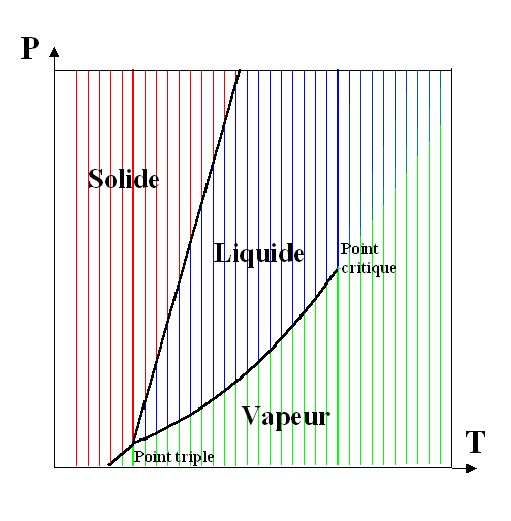
\includegraphics[width=6cm]{pft.jpg}
%  \caption{Diagramme p=f(t)}
%\end{figure}
Il existe deux points caractéristiques sur ce diagramme :
\begin{itemize}
 \item[$\rightarrow$] T : Point triple du corps pur
 \item[$\rightarrow$] C : Point Critique
\end{itemize}
\subsection{Pente des frontières de coexistence}
La pente de la courbe est toujours croissante, c'est à dire qu'une augmention de T impose une augmentation de pression dans un corps pur.\\
Il existe une exception. Pour l'eau, la pente de la frontière Solide $\rightarrow$ Liquide est négative
\subsection{Point Triple : T}
\begin{de}
 T, appelé point triple, correspond au domaine de coexistence des trois phases du corps pur considéré. Ce point est une propriété intrinsèque du corps. C'est le point triple de l'eau pur qui défini l'échelle de température. On le fixe a 273,15 K.
\end{de}
\subsection{Point Critique : C}
\begin{de}
 C est la limite de coexistence des phases liquide et gazeuse d'un corps pur. Au dessus de ce point, on passe de manière continue de l'état gazeuse à l'état liquide sans observer d'état diphasé. On observe ce qu'on appelle un état fluide.
\end{de}
\section{Diagramme p=f(v) de l'équilibre liquide-gaz.\\ Isotherme d'Andrews}
Dans cette étude, v est le volume massique.
%\begin{figure}[h]
%  \centering
%  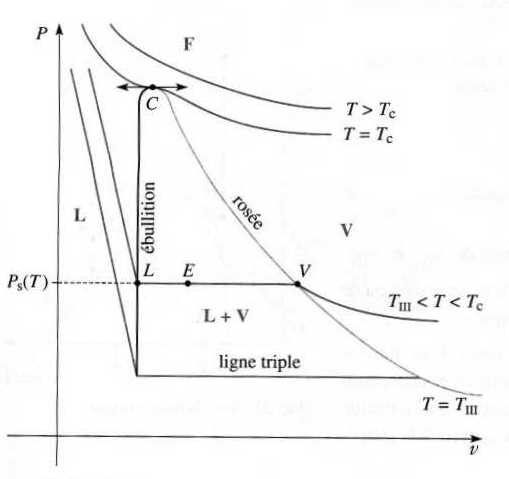
\includegraphics[width=6cm]{isotherme.jpg}
%  \caption{Diagramme p=f(v)}
%\end{figure}\\
Au point L, il y a apparition de la première bulle de Gaz. Au point V, la dernière goutte d'eau se vaporise. Cette évolution s'effectue à pression constante. Cette pression, qui est notée $P_s$(T) ou $\pi_s$(T), est la pression de vapeur saturante. Cette pression augmente avec la température. Ceci est l'illustration que tout système diphasé est monovariante. Ceci est vrai pour T<$T_s$. Pour $T>T_s$, on passe de l'état liquide à l'état gazeux de manière continue, on dit qu'on est dans un état fluide.
\subsection{Propriété du point critique}
\subsubsection{Opalesence Optique}
Au point critique, pour T=$T_c$, $\chi_t$ tend vers $\infty$. Ceci implique donc que la densité du milieu connait de très forte fluctuation, or on montre que l'indice d'un milieu est lié à la densité de celui-ci. Dans ces conditions, le corps pur diffuse de manière particulière la lumière, on appelle ce phénomène opalescence optique.
\subsubsection{Stockage des fluides}
D'après l'équation d'état de l'eau liquide, on à montré qu'une faible augmentation de température, au corps d'une évolution isochore, entrainement une très forte augmentation de pression. Pour cette raison, on stocke les fluides dans un état diphasé. On les stocke dans un volume V supérieur au volume $V_c$ du point critique, car une augmentation de temperature entraine un augmentation de pression relativement faible.
\section{Enthalpie et entropie de transition de phase}
On defini au cours de cette section l'enthalipe et l'entropie au cours de certaine évolution. Cependant, ces deux grandeurs sont toutes deux des fonctions d'états, donc les expressions qui suivent sont vrai pour tout type d'évolution.
\subsection{Enthalpie}
\begin{de}
Dans le cadre d'une évolution isotherme, on a : 
$$\Delta H = ml = L = Q$$
\end{de}
\subsubsection{Chaleur latente}
\begin{de}
 La variation d'enthalpie d'un corps pur au court d'une transition de phase est appelé chaleur latente de transition de phase, notée L.\\
De plus, nous savons que Q est positif pour une transition de phase d'un état ordonné vers un état moins ordonnée. Ce qui implique que dans ce cas, L est positif. Dans la situation inverse, L est négatif, tout comme Q. 
\end{de}
\section{Entropie}
\begin{de}
Dans le cadre d'une évolution isotherme, donc isobare, la variation d'entropie d'une masse m de corps pur est donnée par : 
$$\Delta S= \dfrac{ml}{T}$$
\end{de}
\section{Complément de culture}
\subsection{Évaporation}
Considérons de l'eau. Cette eau se vaporise, à une température $T_0$, jusqu'à atteindre la pression de vapeur saturante, $\pi_s$, qui dépend de T. Dans l'atmosphère, l'eau se vaporise jusqu'à que la pression partielle de l'eau soit égale à $\pi_s$. On défini donc $\tau$, le taux d'hygrométrie, qui est le rapport de la pression partielle de l'eau sur la pression de vapeur saturante :
$$\tau = \dfrac{p(H_2O)}{\pi_s(T_0)}$$
\subsection{Ébullition}
L'ébullition est l'apparition de bulle dans un liquide. La condition d'ébulition est :
\[\left\{\begin{array}{l}
\pi_s(T_0)> p_0 + \rho gh \mbox{ Ébullition}\\
\pi_s(T_0)< p_1 + \rho gh  \mbox{ Pas ébulition} \\
\end{array}\right.\]
avec $p_1>p_0$
\subsection{Etat métastable}
Très souvent, dans les transitions de phases, il existe un retard. On parle durant ce retard d'état métastable. Ce retard s'exprime dans de nombreux phénomène comme : 
\begin{itemize}
 \item[$\rightarrow$] Trainée blanche apres le passage des avions
 \item[$\rightarrow$] Chevaux du lac Ladoga
\end{itemize}

